\documentclass[10pt,a4paper]{article}
\usepackage[top=2.3cm,bottom=1.2cm,left=1.5cm,right=1.5cm]{geometry}
\usepackage[utf8]{inputenc} 
\usepackage[T1]{fontenc}   
\usepackage{indentfirst}
\setlength{\parindent}{2em}
\usepackage{multicol}
\usepackage{setspace}
\usepackage{bm}
\usepackage{pifont}
\usepackage{float}
\usepackage{amssymb}
\usepackage[tbtags]{amsmath} 
\usepackage{tikz}
\usepackage{subcaption}

\usetikzlibrary{arrows.meta}
\tikzset{
    dot/.style={circle, fill, inner sep=1.5pt}, % 定义格点的样式
    main plot/.style={scale=0.7, font=\small} % 定义每个子图的通用样式
}

\usepackage[
    backend=biber,      
    style=numeric-comp, 
    sorting=none        
]{biblatex}
\addbibresource{references.bib} 
\usepackage{hyperref}

\numberwithin{equation}{section}
\renewcommand{\baselinestretch}{1.5}

\newcommand{\ket}[1]{\left| #1 \right\rangle}
\newcommand{\vev}[1]{\left\langle #1 \right\rangle}


\begin{document}
\title{Fusion products of representations of the $\widehat{\mathfrak{sl}_{2}}$ algebra}
\maketitle


\begin{abstract}
    In this thesis, we review the representations appear in the $\widetilde{SL}_{2}(\mathbb{R})$ WZW model and the degenerate representations that are needed 
    to bootstrap this model. We determine fusion rules by solving Ward identities for both spectral flow preserving and violating cases. 
    We then show that the fusion rule is consistant with the proposed fusion rules of the $\widetilde{SL}_{2}(\mathbb{R})$ WZW model.
\end{abstract}

\tableofcontents

\section{Introduction and overview}
The $\widetilde{SL}_{2}(\mathbb{R})$ Wess-Zumino-Witten (WZW) model is a conformal field theory (CFT) with additional 
symmetry of affine Lie algebra $\widehat{\mathfrak{sl}_{2}}$. The study of the $\widetilde{SL}_{2}(\mathbb{R})$ WZW model is motivated by 
its connection with string theory in $AdS_{3}$. However, this model has not been completely solved: the 3-point function is not 
fully known and the crossing symmetry has not been proved yet. \\

















\section{SL(2,R) WZW model}
In this chapter, we introduce the theoretical foundation of the WZW model, especially concentrate on the 
$\widetilde{SL}_{2}(\mathbb{R})$ case. We begin by defining the algebraic structures, and then define fields and representations 
appear in this model. At last, we give the correlation functions that are necessary to solve this model. 

\subsection{Non-abelian affine symmetries}
\subsubsection*{Reminders on Lie algebra}
A Lie algebra is a vector space $\mathfrak{g}$ equipped with a binary operation $\left[\cdot,\cdot \right]:\mathfrak{g}\times \mathfrak{g} \rightarrow \mathfrak{g}$,
known as the Lie bracket, which satisfies the following axioms:
\begin{itemize}
    \item Bilinearity:$\quad \left[ax+by,z \right] = a \left[x,z\right] + b \left[y,z\right],\quad \left[z,ax+by \right] = a \left[z,x\right] + b \left[z,y\right]$.
    \item Antisymmetry:$\quad \left[x,y\right] = - \left[y,x\right]$.
    \item Jacobi identity:$\quad \left[a,\left[b,c\right]\right]+\left[b,\left[c,a\right]\right]+\left[c,\left[a,b\right]\right] = 0$.
\end{itemize}
For a basis of generators $t^{a}$ of $\mathfrak{g}$, the Lie bracket is defined by their commutation relations:
\begin{equation}
    \left[t^{a},t^{b}\right] = f^{ab}_{c} t^{c}.
\end{equation}
The numbers $f^{ab}_{c}$ are called structure constants of the Lie algebra. From these, one can define an invariant symmetric tensor 
called the Killing form: 
\begin{equation}
    K^{ab} = \frac{1}{2g} f^{ac}_{d}f^{bd}_{c},
\end{equation}
where $g$ is the dual Coxeter number of $\mathfrak{g}$. For our the case of $\mathfrak{sl}_{2}$, this number is $g = 2$. And the non-zero Killing form is 
\begin{equation}
    K^{00} = \frac{1}{2}, \quad K^{+-} = K^{-+} = 1.
\end{equation}

A key operator is the quadratic Casimir operator, defined as  
\begin{equation}
    C = K_{ab} t^{a} t^{b},
\end{equation}
which commutes with all Lie algebra generators: $\left[C,t^{a}\right] = 0$. This means that in an irreducible representation, 
the Casimir operator is proportional to the identity. 

For the algebra $\mathfrak{sl}_{2}$, its irreducible representations are labeled by a number $j$, called the spin. 
The eigen value of the Casimir operator is 
\begin{equation}
    C = 2 t^{0} t^{0} + t^{+} t^{-} + t^{-} t^{+} = 2j(j+1).
\end{equation}

\subsubsection*{Symmetry algebra}
We now define the symmetry algebra of the WZW model. 
The $G$ WZW model is a CFT with an infinite-dimensional affine Lie algebra, denoted as $\hat{\mathfrak{g}}_{k}$. 
This algebra is generated by a number of dim$\mathfrak{g}$ of 
holomorphic $\hat{\mathfrak{g}}_{k}$ currents $J^{a}(z)$ through their OPEs,
\begin{equation}
    \boxed{
        J^{a}(z)J^{b}(w) = \frac{kK^{ab}}{(z-w)^{2}} + \frac{f^{ab}_{c} J^{c}(w)}{z-w} + \mathcal{O}(1), \label{OPEJJ}
        }
\end{equation}
where the constant $k$ is the level, which is the most important parameter of the model. 

The modes of the current are defined by 
\begin{equation}
    J^{a}_{n} = \oint \mathrm{d}z \, z^{n} J^{a}(z).
\end{equation}
From the OPEs \eqref{OPEJJ}, we deduce the following commutation relations, 
which formally define the affine Lie algebra $\widehat{\mathfrak{sl}}(2)_{k}$
\begin{equation}
    \boxed{
        \left[ J^{a}_{m}, J^{b}_{n} \right] = f^{ab}_{c} J^{c}_{m+n} + m k K^{ab} \delta_{m+n,0}. \label{CR1}
    }
\end{equation}

\subsubsection*{The Sugawara construction}
We introduce the Sugawara construction for the the energy momentum tensor $T(z)$
\begin{equation}
    \boxed{
        T(z) = \frac{K_{ab}}{2(k-g)} : J^{a}(z) J^{b}(z) : . \label{EM}
        } 
\end{equation}
$T$ is a Virasoro field with central charge $c = \frac{k \mathrm{dim} \mathfrak{g}}{k-g}$. In our case of $\widetilde{SL}_{2}(\mathbb{R})$ 
WZW model, this gives 
\begin{equation}
    \boxed{
        c = \frac{3k}{k-2}
        }
\end{equation}

The Virasoro generators are given by
\begin{equation}
    L_{n} = \frac{K_{ab}}{2(k+g)} : \sum_{m \in \mathbb{Z} } J^{a}_{n-m} J^{b}_{m} :. \label{DefLn}
\end{equation}
Using the commutation relations for the $J^{a}_{n}$ \eqref{CR1}, we can deduce commutation relation between $L_{m}$ and $J^{a}_{n}$:
\begin{equation}
    \boxed{
            \left[ L_{m}, J^{a}_{n} \right] = -n J^{a}_{m+n}. \label{CR2}
    }
\end{equation}

\subsection{Affine primary fields}
An affine primary field $\phi^{\mathcal{j}}(z)$ associated with representation $\mathcal{R}^{j}$ is defined by its OPE with current field 
$J^{a}(y)$:
\begin{equation}
    \boxed{
        J^{a}(y) \phi^{j}(z) \sim \frac{-(t^{a})^{T} \phi^{j}(z)}{y-z} + \mathcal{O}(1), \label{OPEJPhi}
    }
\end{equation}
where $t^{a}$ is the generator of Lie algebra $\mathfrak{sl}_{2}$. This OPE involves the transposition of Lie algebra generators, which 
flips the sign of commutation relations. Hence we need a minus sign in the OPE. The minus sign also ensures the associativity of 
the OPE $J^{a}J^{b} \phi$. 

Followed from the Sugawara construction, an affine primary field is also a Virasoro primary field. 
The OPE between $T(y)$ and $\phi^{j}(z)$ can be obtained from the Sugawara construction \ref{EM}:
\begin{equation}
    T^{y} \phi^{j}(z) = \frac{K_{ab} (t^{a})}{k+g} \left( \frac{\frac{1}{2} t^{b} \phi^{j}(z)}{(y-z)^{2}} - \frac{\left(J^{b} \phi^{j}\right)(z)}{y-z} \right) + \mathcal{O}(1).
\end{equation}
The conformal dimension of an affine primary field $\phi^{j}(x)$ is propotional to the Casimir operator $C = K_{ab} t^{a} t^{b}$ :
\begin{equation}
    \boxed{
        \Delta_{j} = \frac{C(j)}{2(k+g)} = \frac{j(j+1)}{k+g}.
    }
\end{equation}

Based on the state-field correspondence, the field $\phi^{j}(z)$ corresponds to an affine primary state $\ket{v^{j}}$ in the Hilbert spece. 
The OPE \ref{OPEJPhi} implies the action of currents modes on this state:
\begin{equation}
    \left\{
        \begin{aligned}
            J^{a}_{n>0} \ket{v^{j}} &= 0,\\
            J^{a}_{0} \ket{v^{j}} &= - t^{a} \ket{v^{j}}.
        \end{aligned}
    \right.
\end{equation}

\subsubsection*{Isospin variables}
For practical calculations, especially for solving Ward identities, it is useful to realize the abstract action of the generators 
$t^{a}$ as differential operators acting on functions. We introduce the isospin variables and 
represent the fields as functions of the isospin variables, 
where $t^{a}$ acts on primary fields as differential operators $D^{j}(t^{a})$. We introduce two important bases:

$\mathbf{x-basis}$: In this basis, a field is represented as a function $\phi^{j}_{x}$, and $t^{a}$ acts as 
\begin{equation}
    \left\{
        \begin{aligned}
            D^{j}_{x}(t^{+}) &= x^{2} \partial_{x} - 2 j x, \\
            D^{j}_{x}(t^{0}) &= x \partial_{x} - j, \\
            D^{j}_{x}(t^{-}) &= - \partial_{x}.
        \end{aligned}
    \right. \label{Diffx}
\end{equation}
Because of the transposition in \ref{OPEJPhi}, in the isospin formalism the generator $J^{a}_{0}$ acts as 
\begin{equation}
    J^{a}_{0} J^{b}_{0} \phi^{j}_{x}(z) = \left( -D^{j}_{x}\left(t^{b}\right) \right) \left( -D^{j}_{x}\left(t^{a}\right) \right) \phi^{j}_{x}(z).
\end{equation}

$\mathbf{\mu-basis}$: The $t^{a}$ acts as 
\begin{equation}
    \left\{
        \begin{aligned}
            D^{j}_{x}(t^{+}) &= \mu \partial_{\mu}^{2} - \frac{j(j+1)}{\mu}, \\
            D^{j}_{x}(t^{0}) &= -\mu \partial_{\mu}, \\
            D^{j}_{x}(t^{-}) &= -\mu.
        \end{aligned}
    \right. \label{Diffmu}
\end{equation}

The $x$-basis field $\phi^{j}_{x}(z)$ and $\mu$-basis field $\phi^{j}_{\mu}(z)$ are related by the Fourier transformation 
\begin{equation}
    \phi^{j}_{x}(z) \sim \int \mathrm{d} \mu \, \mu^{-j-1} \mathrm{e}^{\mu x} \phi^{j}_{\mu}(z).
\end{equation}

Another important basis is the $\mathbf{m-basis}$, where the where the Casimir $C$ and $J^{0}_{0}$ are diagonalized. We denote the 
state in $m$-basis to be $\ket{j,m}$. The action of 
$J^{\pm}_{0}$ on $\ket{j,m}$ is defined to be:
\begin{equation}
    \begin{aligned}
        J^{-}_{0} \ket{j,m} &= (-j-1+m)\ket{j,m-1}, \\
        J^{0}_{0} \ket{j,m} &= m \ket{j,m} \\
        J^{+}_{0} \ket{j,m} &= (-j-1-m)\ket{j,m+1}. \label{Jpm}
    \end{aligned}
\end{equation}
The field $\phi^{j}_{m}(z)$ corresponding to the state $\ket{j,m}$ is related to the $\mu$-basis field by 
\begin{equation}
    \phi^{j}_{m}(z) \sim \int \mathrm{d} \mu \, \mu^{-m} \phi^{j}_{\mu}(z).
\end{equation}


\subsection{Irreducible representations}
\subsubsection*{Irreducible representations of \texorpdfstring{$\mathfrak{sl}_{2}$}{Lg}}
For a given affine Lie algebra $\widehat{\mathfrak{g}}$, we define the horizontal algebra to be the subalgebra generated by zero-mode 
generators $J^{a}_{0}$. The central extension in \ref{CR1} vanishes for $m = 0$, hence the subalgebra is isomorphic to the underlying 
Lie algebra $\mathfrak{g}$. An irreducible representation $\mathcal{R}$ of $\mathfrak{g}$ can be naturally extended to an affine 
highest-weight representation $\widehat{\mathcal{R}}$, which is not necessarily irreducible though.

We work in the m-basis. From \ref{Jpm}, we find two specific state, namely $\ket{j,\pm}$. They satisfy the following vanishing condition:
\begin{equation}
    J^{\pm} \ket{j,\pm j} = 0.
\end{equation}
Hence we can classify different representations by the existence of these states.

The unitary representations appear in the spectrum can be classified into several series:
\begin{itemize}
    \item Principle continuous series $\mathcal{C}^{j}_{\alpha}$. They are labeled by spin $j \in -\frac{1}{2} + \mathrm{i} \mathbb{R}_{+}$ and 
    a real number $\alpha \in \left(0,1\right)$. The eigenvalue $m$ of $J^{0}_{0}$ is unbounded both above and below, taking values $m \in \alpha + \mathbb{R}$.
    \item Discrete series $\mathcal{D}^{j,\pm}$. They are labeled by real spin $j \in (-\infty,-\frac{1}{2})$ and contain the state 
    $\ket{j,\mp j}$ respectively. Hence the spectrum is either bounded from below and from above.
\end{itemize}
Another crucial but non-unitary class of representations are the finite dimensional representations $\mathcal{E}^{j}$, which contain 
both $\ket{j,j}$ and $\ket{j,-j}$. They exist only 
when $j$ takes integer or half-integer values $j \in \mathbb{N}/2$, where $m$ takes values in $\{-j, -j+\frac{1}{2},\cdots,j-\frac{1}{2},j \}$.
We summarize the properties of these representations in the following table.
\begin{center}
    \begin{tabular}{|l|l|l|l|}
        \hline
        Representations&Parameter values&Eigenvalues of $J^{0}_{0}$&Conjugate representation\\
        \hline
        $\mathcal{C}^{j}_{\alpha}$ & $j \in -\frac{1}{2} + i \mathbb{R}_{+} $, $\alpha \in \mathbb{R}$ mod $\mathbb{Z}$& $\alpha + \mathbb{Z}$&$\mathcal{C}^{j}_{-\alpha}$\\
        $\mathcal{D}^{j,+}$ & $j \in (-\infty,-\frac{1}{2}) $& $-j + \mathbb{N}$&$\mathcal{D}^{j,-}$\\
        $\mathcal{D}^{j,-}$ & $j \in (-\infty,-\frac{1}{2}) $& $j - \mathbb{N}$&$\mathcal{D}^{j,+}$\\
        $\mathcal{E}^{j}$ & $j \in \mathbb{N}/2 $ & $\left\{-j,-j+\frac{1}{2}, \cdots, j-\frac{1}{2},j \right\}$&$\mathcal{E}^{j}$\\
        \hline
    \end{tabular}
\end{center}
From the above representations of $\mathfrak{sl}_{2}$, we can naturally induce the corresponding representations of $\widehat{\mathfrak{sl}_{2}}$. 
We plot the states by their eigenvalues of $L_{0}$ and $J^{0}_{0}$ in \ref{fig:irrep}.

\begin{figure}[htbp]
    \centering 
    \begin{subfigure}[b]{0.48\textwidth}
        \centering
        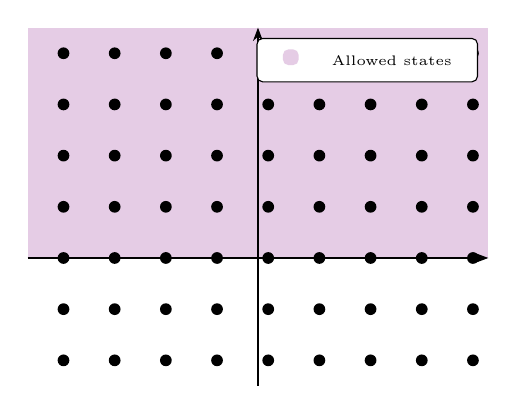
\begin{tikzpicture}[scale=0.65, font=\small]
            \def\xmin{-4.5} \def\xmax{4.5} \def\ymin{-2.5} \def\ymax{4.5}
            \clip (\xmin, \ymin) rectangle (\xmax, \ymax);
            
            \fill[violet!20] (\xmin, 0) rectangle (\xmax, \ymax);
            
            \draw[-{Stealth[]}] (\xmin, 0) -- (\xmax, 0) node[anchor=north west] {$J_0^0$};
            \draw[-{Stealth[]}] (0, \ymin) -- (0, \ymax) node[anchor=south east] {$L_0$};
            \foreach \x in {-4,...,4} {\foreach \y in {-2,...,4} {\node[dot] at (\x+0.2,\y) {};}}
                        
            \node[draw, fill=white, rounded corners=2pt, align=left, anchor=north east, font=\tiny] at (\xmax-0.2, \ymax-0.2) {
                \begin{tabular}{rl}\tikz\fill[violet!20](0,0)rectangle(0.2,0.2);&Allowed states\end{tabular}};
        \end{tikzpicture}
        \caption{$\widehat{\mathcal{C}}^{j}_{\alpha}$}
        \label{fig:C}
    \end{subfigure}
    \hfill 
    % (b) 右上角子图: V形边界
    \begin{subfigure}[b]{0.48\textwidth}
        \centering
        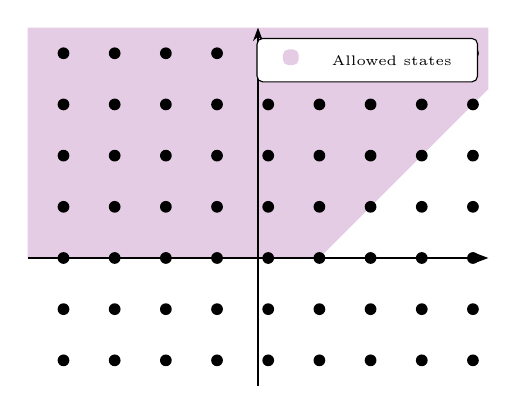
\begin{tikzpicture}[scale=0.65, font=\small]
            \def\xmin{-4.5} \def\xmax{4.5} \def\ymin{-2.5} \def\ymax{4.5}
            \clip (\xmin, \ymin) rectangle (\xmax, \ymax);

            \fill[violet!20] (\xmin, 0) -- (1.2, 0) -- (\xmax, \xmax-1.2) -- (\xmax, \ymax) -- (\xmin, \ymax) -- cycle;
            
            \draw[-{Stealth[]}] (\xmin, 0) -- (\xmax, 0) node[anchor=north west] {$J_0^3$};
            \draw[-{Stealth[]}] (0, \ymin) -- (0, \ymax) node[anchor=south east] {$L_0$};
            \foreach \x in {-4,...,4} {\foreach \y in {-2,...,4} {\node[dot] at (\x+0.2,\y) {};}}            
            
            \node[draw, fill=white, rounded corners=2pt, align=left, anchor=north east, font=\tiny] at (\xmax-0.2, \ymax-0.2) {
                \begin{tabular}{rl}\tikz\fill[violet!20](0,0)rectangle(0.2,0.2);&Allowed states\end{tabular}};
        \end{tikzpicture}
        \caption{$\widehat{\mathcal{D}}^{j,-}$}
        \label{fig:D-}
    \end{subfigure}

    \vspace{1cm}

    %=====================================================
    % --- 第二行 ---
    %=====================================================

    % (c) 左下角子图: 倒V形边界
    \begin{subfigure}[b]{0.48\textwidth}
        \centering
        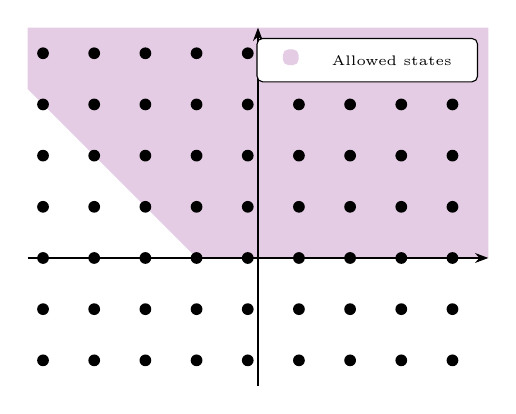
\begin{tikzpicture}[scale=0.65, font=\small]
            \def\xmin{-4.5} \def\xmax{4.5} \def\ymin{-2.5} \def\ymax{4.5}
            \clip (\xmin, \ymin) rectangle (\xmax, \ymax);

            \fill[violet!20] (\xmin, -\xmin-1.2) -- (-1.2, 0) -- (\xmax, 0) -- (\xmax, \ymax) -- (\xmin, \ymax) -- cycle;

            \draw[-{Stealth[]}] (\xmin, 0) -- (\xmax, 0) node[anchor=north west] {$J_0^3$};
            \draw[-{Stealth[]}] (0, \ymin) -- (0, \ymax) node[anchor=south east] {$L_0$};
            \foreach \x in {-4,...,4} {\foreach \y in {-2,...,4} {\node[dot] at (\x-0.2,\y) {};}}
                                    
            \node[draw, fill=white, rounded corners=2pt, align=left, anchor=north east, font=\tiny] at (\xmax-0.2, \ymax-0.2) {
                \begin{tabular}{rl}\tikz\fill[violet!20](0,0)rectangle(0.2,0.2);&Allowed states\end{tabular}};
        \end{tikzpicture}
        \caption{$\widehat{\mathcal{D}}^{j,+}$}
        \label{fig:D+}
    \end{subfigure}
    \hfill
    % (d) 右下角子图: 最终修正的复杂边界
    \begin{subfigure}[b]{0.48\textwidth}
        \centering
        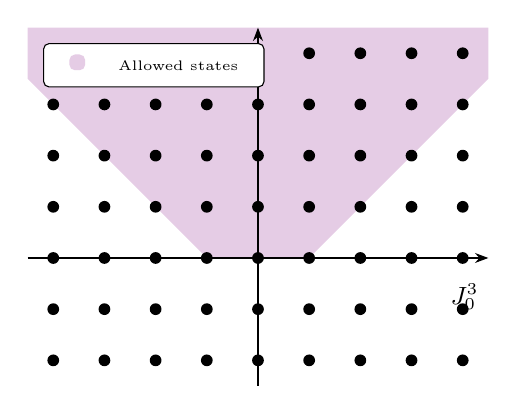
\begin{tikzpicture}[scale=0.65, font=\small]
            \def\xmin{-4.5} \def\xmax{4.5} \def\ymin{-2.5} \def\ymax{4.5}
            \clip (\xmin, \ymin) rectangle (\xmax, \ymax);

            \fill[violet!20] (\xmin, -\xmin-1) -- (-1, 0) -- (1, 0) -- (\xmax, \xmax-1) -- (\xmax, \ymax) -- (\xmin, \ymax) -- cycle;

            \draw[-{Stealth[]}] (\xmin, 0) -- (\xmax, 0) node[anchor=north east, yshift=-2mm] {$J_0^3$};
            \draw[-{Stealth[]}] (0, \ymin) -- (0, \ymax) node[anchor=south east] {$L_0$};
            \foreach \x in {-4,...,4} {\foreach \y in {-2,...,4} {\node[dot] at (\x,\y) {};}}
            
            \node[draw, fill=white, rounded corners=2pt, align=left, anchor=north west, font=\tiny] at (\xmin+0.3, \ymax-0.3) {
                \begin{tabular}{rl}\tikz\fill[violet!20](0,0)rectangle(0.2,0.2);&Allowed states\end{tabular}};
        \end{tikzpicture}
        \caption{$\widehat{\mathcal{E}}^{j}$}
        \label{fig:E}
    \end{subfigure}

    \caption{The spectra of irreducible representations of $\widehat{\mathfrak{sl}_{2}}$}
    \label{fig:irrep}
\end{figure}

\subsubsection*{Spectral flow}
The Spectral flow is a family $(\rho_{\omega})_{\omega \in \mathbb{Z}}$ of automorphisms of $\widehat{\mathfrak{sl}}_{2}$
satisfying $\rho_{\omega_{1}} \circ \rho_{\omega_{2}}  = \rho_{\omega_{1} + \omega_{2}}$, which are defined by 
\begin{equation}
    \begin{aligned}
        \rho_{\omega}(J^{\pm}_{m}) & = J^{\pm}_{m \pm \omega},\\
        \rho_{\omega}(J^{0}_{m}) & = J^{0}_{m} + \frac{1}{2} k \omega \delta_{m,0}.
    \end{aligned}
\end{equation}
According to the Sugawara construction \ref{DefLn}, the spectral flow of Virasoro generators is 
\begin{equation}
    \rho_{\omega}(L_{m}) = L_{m} + \omega J^{0}_{m} + \frac{1}{4} k n^{2} \delta_{m,0}.
\end{equation}
Hence the conformal dimension of a spectral flowed primary field $\phi^{j,\omega}_{m}(z)$ is 
\begin{equation}
    \Delta^{j,\omega}_{m} = \Delta_{j} - \omega m - \frac{1}{4} k n^{2}. \label{SpecFlowConDim}
\end{equation}

A representation $\widehat{\mathcal{R}} $ provides the action of generators $J^{a}_{n}$ on vector space $V$. Based on this representation, 
we define the spectral flowed representation $\rho_{\omega}\left(\hat{\mathcal{R}}\right)$. The spectral flowed representation acts on the 
same vector space $V$, but the action of generators $J^{a}_{n}$ is defined to be $\rho_{-\omega}\left(J^{a}_{n}\right)$. 

For clarity in calculations, we label the states in $\rho_{\omega}\left(\hat{\mathcal{R}}\right)$ by $\ket{j,m,\omega}$. The definition 
of the action of generators $J^{a}_{n}$ leads to
\begin{equation}
    J^{a}_{n} \ket{j,m,\omega} \equiv \rho^{-\omega} \left(J^{a}_{n}\right) \ket{j,m},
\end{equation}
where we omit the label $0$ in state $\ket{j,m,0}$ for simplicity. 
The conjugate representation of $\rho_{n} \left(\hat{\mathcal{R}} \right)$ is 
\begin{equation}
    \rho_{\omega} \left( \hat{\mathcal{R}} \right)^{*} = \rho_{-\omega} \left(\hat{\mathcal{R}}^{*} \right)
\end{equation}
In addition, it's believed that the spectral flow commutes with fusion \cite{Gaberdiel:2001ny}, 
\begin{equation}
    \rho_{\omega_{1}} \left(\hat{\mathcal{R}}\right) \times \rho_{\omega_{2}} \left(\mathcal{R'}\right) = \rho_{\omega_{1} + \omega_{2}} \left(\hat{\mathcal{R}}\times \mathcal{R'}\right). \label{SpecFus}
\end{equation}

Let's consider the action of spectral flow on affine highest-weight representations. We introduce the following notation 
\begin{equation}
    \begin{aligned}
        \hat{\mathcal{C}}^{j,\omega} &= \rho_{\omega} \left( \hat{\mathcal{C}}^{j} \right),\\
        \hat{\mathcal{D}}^{j, \frac{1}{2} + \omega} &= \rho_{\omega} \left( \hat{\mathcal{D}}^{j, +} \right).
    \end{aligned}
\end{equation}
From \ref{SpecFlowConDim}, we find the conformal dimension of states in $\hat{\mathcal{C}}^{j,\omega}$ of non-zero $\omega$ are not bounded 
from below. Hence it cannot be an affine highest-weight representation.

On the other hand, the representations $\hat{\mathcal{D}}^{j,\pm}$ are characterized by the existence of state $\ket{j,\mp j}$, 
which satisfy the following conditions:
\begin{equation}
    J^{a}_{n>0} \ket{j,\pm j} = J^{\pm}_{0} \ket{j,\pm j} = (J^{0}_{0} \mp j) \ket{j,\pm j} =0.
\end{equation}
In particular, we notice that 
\begin{equation}
    \begin{aligned}
        J^{+}_{n \geq 0} \ket{j,-j,-1} &= J^{+}_{n+1} \ket{j,-j}  = 0, \\
        J^{0}_{n > 0} \ket{j,-j,-1} & =  J^{0}_{n}\ket{j,-j} = 0,\\
        \left(J^{0}_{0} - \frac{k}{2} +j \right) & = \left( J^{0}_{0} + j \right) \ket{j,-j} = 0,
        J^{-}_{n>0} \ket{j,-j,-1} &= J^{-}_{n-1} \ket{j,-j}   =  0.
    \end{aligned}
\end{equation}
Hence we find $\ket{j,-j,-1} = \ket{\frac{k}{2}-j, \frac{k}{2}-j}$, and 
\begin{equation}
    \hat{\mathcal{D}}^{j,-\frac{1}{2}} = \rho_{-1} \left( \hat{\mathcal{D}}^{j,+} \right) = \hat{\mathcal{D}}^{\frac{k}{2}-j,-}.
\end{equation}
Now we can use out new notation to write the discrete series representations as 
\begin{equation}
    \widehat{\mathcal{D}}^{j,+} = \widehat{\mathcal{D}}^{j,\frac{1}{2}},\quad \widehat{\mathcal{D}}^{j,-} = \widehat{\mathcal{D}}^{\frac{k}{2}-j,-\frac{1}{2}}.
\end{equation}

Since the eigenvalue of $L_{0}$ are related to $m$, the spectrum of spectral flowed representations 
are twisted. We plot the spectrum of $\widehat{\mathcal{C}}^{j,1}_{\alpha}$ and $\widehat{\mathcal{D}}^{\frac{k}{2}-j, -\frac{1}{2}}$ 
in \ref{fig:irrepSF}.

\begin{figure}[htbp]
    \centering 
    \begin{subfigure}[b]{0.48\textwidth}
        \centering
        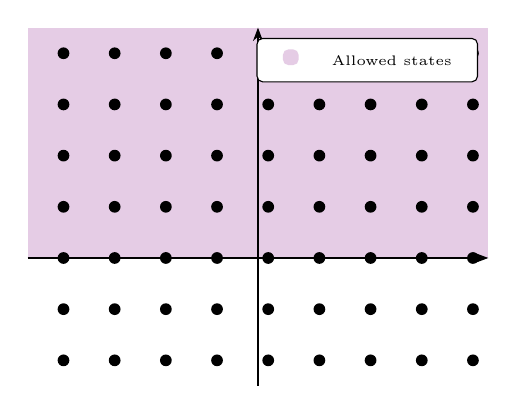
\begin{tikzpicture}[scale=0.65, font=\small]
            \def\xmin{-4.5} \def\xmax{4.5} \def\ymin{-2.5} \def\ymax{4.5}
            \clip (\xmin, \ymin) rectangle (\xmax, \ymax);
            
            \fill[violet!20] (\xmin, 0) rectangle (\xmax, \ymax);
            
            \draw[-{Stealth[]}] (\xmin, 0) -- (\xmax, 0) node[anchor=north west] {$J_0^0$};
            \draw[-{Stealth[]}] (0, \ymin) -- (0, \ymax) node[anchor=south east] {$L_0$};
            \foreach \x in {-4,...,4} {\foreach \y in {-2,...,4} {\node[dot] at (\x+0.2,\y) {};}}
                        
            \node[draw, fill=white, rounded corners=2pt, align=left, anchor=north east, font=\tiny] at (\xmax-0.2, \ymax-0.2) {
                \begin{tabular}{rl}\tikz\fill[violet!20](0,0)rectangle(0.2,0.2);&Allowed states\end{tabular}};
        \end{tikzpicture}
        \caption{$\widehat{\mathcal{C}}^{j}_{\alpha}$}
        \label{fig:C0}
    \end{subfigure}
    \hfill 
%second picture at up-right corner
    \begin{subfigure}[b]{0.48\textwidth}
        \centering
        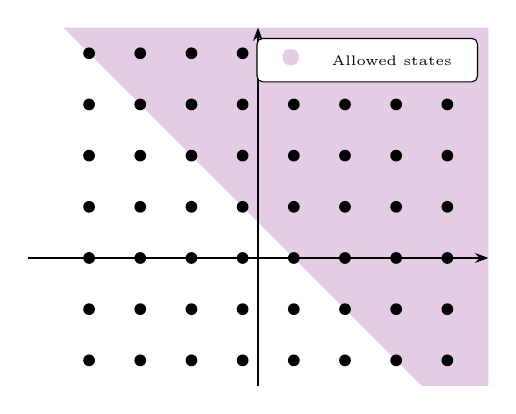
\begin{tikzpicture}[scale=0.65, font=\small]
            \def\xmin{-4.5} \def\xmax{4.5} \def\ymin{-2.5} \def\ymax{4.5}
            \clip (\xmin, \ymin) rectangle (\xmax, \ymax);

            \fill[violet!20] (-\ymax+0.7, \ymax) -- (-\ymin+0.7, \ymin) -- (\xmax, \ymin) -- (\xmax, \ymax) -- cycle;
            
            \draw[-{Stealth[]}] (\xmin, 0) -- (\xmax, 0) node[anchor=north west] {$J_0^3$};
            \draw[-{Stealth[]}] (0, \ymin) -- (0, \ymax) node[anchor=south east] {$L_0$};
            \foreach \x in {-4,...,4} {\foreach \y in {-2,...,4} {\node[dot] at (\x+0.2+0.5,\y) {};}}            
            
            \node[draw, fill=white, rounded corners=2pt, align=left, anchor=north east, font=\tiny] at (\xmax-0.2, \ymax-0.2) {
                \begin{tabular}{rl}\tikz\fill[violet!20](0,0)rectangle(0.2,0.2);&Allowed states\end{tabular}};
        \end{tikzpicture}
        \caption{$\widehat{\mathcal{C}}^{j,1}_{\alpha}$}
        \label{fig:C1}
    \end{subfigure}

    \vspace{1cm}

    %=====================================================
    % --- 第二行 ---
    %=====================================================

    \begin{subfigure}[b]{0.48\textwidth}
        \centering
        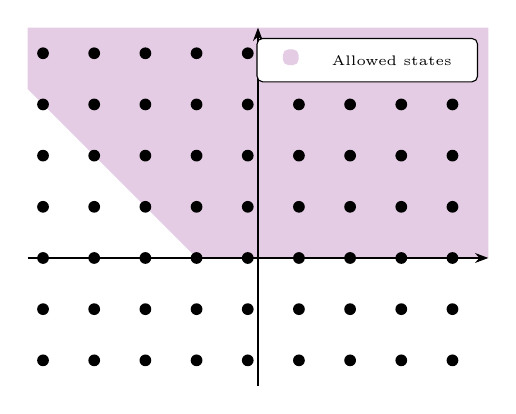
\begin{tikzpicture}[scale=0.65, font=\small]
            \def\xmin{-4.5} \def\xmax{4.5} \def\ymin{-2.5} \def\ymax{4.5}
            \clip (\xmin, \ymin) rectangle (\xmax, \ymax);

            \fill[violet!20] (\xmin, -\xmin-1.2) -- (-1.2, 0) -- (\xmax, 0) -- (\xmax, \ymax) -- (\xmin, \ymax) -- cycle;

            \draw[-{Stealth[]}] (\xmin, 0) -- (\xmax, 0) node[anchor=north west] {$J_0^3$};
            \draw[-{Stealth[]}] (0, \ymin) -- (0, \ymax) node[anchor=south east] {$L_0$};
            \foreach \x in {-4,...,4} {\foreach \y in {-2,...,4} {\node[dot] at (\x-0.2,\y) {};}}
                                    
            \node[draw, fill=white, rounded corners=2pt, align=left, anchor=north east, font=\tiny] at (\xmax-0.2, \ymax-0.2) {
                \begin{tabular}{rl}\tikz\fill[violet!20](0,0)rectangle(0.2,0.2);&Allowed states\end{tabular}};
        \end{tikzpicture}
        \caption{$\widehat{\mathcal{D}}^{j,\frac{1}{2}}$}
        \label{fig:D 1/2}
    \end{subfigure}
    \hfill
%fourth picture at down-right corner
    \begin{subfigure}[b]{0.48\textwidth}
        \centering
        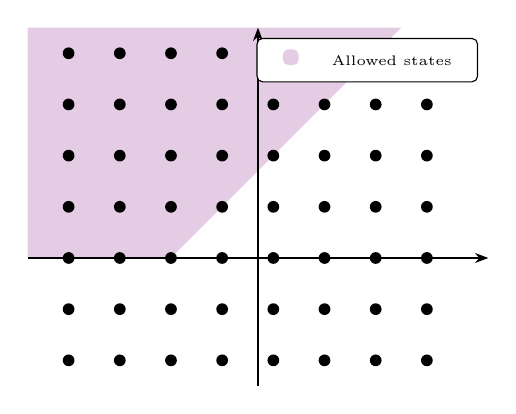
\begin{tikzpicture}[scale=0.65, font=\small]
            \def\xmin{-4.5} \def\xmax{4.5} \def\ymin{-2.5} \def\ymax{4.5}
            \clip (\xmin, \ymin) rectangle (\xmax, \ymax);

            \fill[violet!20] (\xmin, 0) -- (-1.7, 0) -- (\ymax-1.7, \ymax) -- (\xmin, \ymax) -- cycle;
            
            \draw[-{Stealth[]}] (\xmin, 0) -- (\xmax, 0) node[anchor=north west] {$J_0^3$};
            \draw[-{Stealth[]}] (0, \ymin) -- (0, \ymax) node[anchor=south east] {$L_0$};
            \foreach \x in {-4,...,4} {\foreach \y in {-2,...,4} {\node[dot] at (\x-0.7,\y) {};}}            
            
            \node[draw, fill=white, rounded corners=2pt, align=left, anchor=north east, font=\tiny] at (\xmax-0.2, \ymax-0.2) {
                \begin{tabular}{rl}\tikz\fill[violet!20](0,0)rectangle(0.2,0.2);&Allowed states\end{tabular}};
        \end{tikzpicture}
        \caption{$\widehat{\mathcal{D}}^{\frac{k}{2}-j, -\frac{1}{2}}$}
        \label{fig:D 1/2-1}
    \end{subfigure}

    \caption{Spectral flowed irreducible representations}
    \label{fig:irrepSF}
\end{figure}

\subsection{Correlation functions}

\subsubsection*{Ward identities}
The OPE \ref{OPEJJ} implies the behaviour of $J^{a}(z)$ near $y = \infty$:
\begin{equation}
    \boxed{
        J^{a}(y) \underset{y \rightarrow \infty}{=} \mathcal{O}\left(\frac{1}{y^{2}}\right)
    }
\end{equation}
Consider a set of fields $\phi^{\sigma_{i}}(z_{i})$, and a meromorphic function $\epsilon(y)$ such that
$\epsilon(y) \underset{y \rightarrow \infty}{=} \mathcal{O}\left(1\right) $. Suppose $\epsilon(y)$
has no poles outside $\left\{z_{1},\cdots,z_{N} \right\}$, we have 
\begin{equation}
    \oint_{\infty} \mathrm{d} y \, \epsilon(y) \vev{J^{a}(y) \prod_{i} \phi^{\sigma}(z_{i})} = 0. \label{WardId}
\end{equation}
In case of $\epsilon(y) = 1$, we obtain the global Ward identities:
\begin{equation}
    \vev{\sum_{i} \left(J^{a}_{0}\right)^{(z_{i})} \prod_{i} \phi^{\sigma_{i}}(z_{i})} = 0,
\end{equation}
where $\left(J^{a}_{0}\right)^{(z_{i})}$ means the operator acts only on the $i$th field. Especially, if all the fields are affine primary 
fields, the global Ward identities reduce to 
\begin{equation}
    \sum_{i} D^{j_{i}}_{x}(t^{a}) \vev{\prod \phi^{j_{i}}_{x_{i}}(z_{i})} = 0. \label{GlobalWard}
\end{equation}
On the other hand, if we take $\epsilon(y) = \frac{1}{(y-z_{i})^{n}}$ and assume all fields but possibilily the field at 
$z_{i}$ to be affine primary fields, we find the following local Ward identities:
\begin{equation}
    \vev{J^{a}_{-n} \phi^{\sigma_{i}}(z_{i}) \prod_{k \neq i} \phi^{j_{k}}_{x_{k}}(z_{k})} = \sum_{k\neq i} \frac{D^{j_{k}}_{x}(t^{a})}{(z_{k}-z_{i})^{n}} \vev{ \phi^{\sigma_{i}}(z_{i}) \prod_{k \neq i} \phi^{j_{k}}_{x_{k}}(z_{k})} \label{LocalWard}
\end{equation}

\subsubsection*{Three-point functions}
So far, we have only considered the chiral field $\phi^{j}(z)$ belongs to some representation $\widehat{\mathcal{R}^{j}}$ of 
$\widehat{\mathfrak{sl}_{2}}$. However, since the SL(2,R) WZW model is CFT with $\widehat{\mathfrak{sl}_{2}}\times\widehat{\mathfrak{sl}_{2}}$ 
symmetry, the physical field $\phi^{j}(z,\bar{z})$ transforms under both $\widehat{\mathfrak{sl}_{2}}$ algebras. One may assume that 
the physical fields are a product $\phi^{j}(z,\bar{z}) \sim \phi^{j}(z)\phi^{j}(\bar{z})$ of chiral fields. However, this chiral 
factorization fails at the level of zero modes. Hence we need to construct the correlation functions with both holomorphic and anti-holomorphic 
part.

When considreing both the left-moving and right-moving part, the transformation between $x$-basis and $\mu$-basis is then given by 
\begin{equation}
    \phi^{j}_{x,\bar{x}}(z,\bar{z}) = \int \mathrm{d}^{2} \mu \, |\mu|^{-2j-2} \mathrm{e}^{\mu x - \bar{\mu} \bar{x}} \phi^{j}_{\mu,\bar{\mu}}(z,\bar{z}).
\end{equation}
The fields in $m$-basis are related to the $\mu$-basis fields by 
\begin{equation}
    \phi^{j}_{m,\bar{m}}(z,\bar{z}) = N^{j}_{m,\bar{m}} \int \frac{\mathrm{d}^{2} \mu }{|\mu|^{2}} \, \mu^{-m} \bar{\mu}^{-\bar{m}} \phi^{j}_{\mu,\bar{\mu}} (z,\bar{z}).
\end{equation}
where we use the following notation:
\begin{equation}
    \left| F(z,m) \right|^{2} = F(z,m) \times F(z\rightarrow \bar{z}, m \rightarrow \bar{m}).
\end{equation}

The 3-point functions with only affine primary fields can be determined from the global Ward identities \ref{GlobalWard}. 
In x-basis, we find the solution to be:
\begin{equation}
    \begin{aligned}
            \vev{\phi^{j_{1}}_{x_{1},\bar{x}_{1}}(z_{1},\bar{z}_{1}) \phi^{j_{2}}_{x_{2},\bar{x}_{2}}(z_{2},\bar{z}_{2}) \phi^{j_{3}}_{x_{3},\bar{x}_{3}}(z_{3},\bar{z}_{3})} =
            |z_{12}|^{-2 \Delta_{12}^{3}} |z_{23}|^{-2 \Delta_{23}^{1}} |z_{31}|^{-2 \Delta_{31}^{2}}
                 \times D \left[\begin{array}{ccc}
    j_{1} & j_{2} & j_{3} \\
    x_{1} & x_{2} & x_{3}
    \end{array} \right] C(j_{1},j_{2},j_{3}),
    \end{aligned} \label{3pointfuncx}
\end{equation}
where $z_{ij} = z_{i} - z_{j}$ and $\Delta^{K}_{I} = \sum_{i \in I} \Delta_{j_{i}} - \sum_{k \in K} \Delta_{j_{k}}$. The structure constant 
$C(j_{1},j_{2},j_{3})$ is not fully determined yet. The x-dependence is included in factor $D$:
\begin{equation}
    D \left[\begin{array}{ccc}
    j_{1} & j_{2} & j_{3} \\
    x_{1} & x_{2} & x_{3}
    \end{array} \right] = |x_{12}|^{2 j_{12}^{3}} |x_{23}|^{2 j_{23}^{1}} |x_{31}|^{2 j_{31}^{2}}.
\end{equation}
In $\mu$-basis, the corresponding $D$ is 
\begin{equation}
    \begin{aligned}
        D \left[\begin{array}{ccc}
        j_{1} & j_{2} & j_{3} \\
        \mu_{1} & \mu_{2} & \mu_{3}
        \end{array} \right] = & \pi |\mu_{2}|^{-2 j_{1} - 2 j_{3} - 2} |\mu_{1}|^{2j_{1} + 2} |\mu_{3}|^{2j_{3} + 2} \\
                            & \times \left[\frac{\gamma(j_{23}^{1} + 1) \gamma(j_{13}^{2} + 1)}{\gamma(-j_{123}-1) \gamma(2j_{3}+2)} {}_{2} \mathcal{F}_{1} (j_{123} +2, j_{13}^{2} +1, 2j_{3} + 2, -\frac{\mu_{3}}{\mu_{2}}) \right.\\
                            &\quad + \left. \left| \frac{-\mu_{3}}{\mu_{2}}\right|^{-2(2j_{3}+1)} \frac{\gamma(j_{12}^{3} + 1)}{\gamma(-2 j_{3})} {}_{2} \mathcal{F}_{1} (-j_{23}^{1}, j_{12}^{3} +1, -2j_{3}, -\frac{\mu_{3}}{\mu_{2}}) \right]
    \end{aligned}
\end{equation}
where ${}_{2} \mathcal{F}_{1}$ is the product of two hypergeometric functions, 
\begin{equation}
    {}_{2}\mathcal{F}_{1}(a,b,c,z) = F(a,b,c,z) \times F(a,b,c,\bar{z}).
\end{equation}
The factor $\gamma$ is defined by the gamma function 
\begin{equation}
    \gamma(x) = \frac{\Gamma(x)}{\Gamma(1-x)}.
\end{equation}

\subsubsection*{Three-point functions with spectral flow violating}
So far we have only discussed the 3-point function with affine primary fields, by which we can determine the fusion rule where the 
spectral flow is preserved. However, the spectral flow is not necessarily preserved under the fusion. 
Actually, in $n$-point function, the spectral flow can violate by at most $n-2$ units. To understand the full set of fusion rules, 
we must therefore consider these spectral flow-violating correlation functions.

The simplest non-trivial case is a three-point function where the total spectral flow is $\sum_{i} \omega_{i} = \pm 1$. 
Let us consider the case where one field is flowed, e.g., $\vev{\phi^{j_{1}}(z_{1}) \phi^{j_{2}}(z_{2}) \phi^{j_{3},-1}(z_{3})}$. 

The $J^{0}_{0}$ global Ward identities now leads to the following selection rule: 
\begin{equation}
    m_{1} + m_{2} + m_{3} + \frac{k}{2} = 0.
\end{equation}
Since $J^{+}_{0} \phi^{j_{3},-1}(z) = \rho_{-1} \left( J^{+}_{1} \phi^{j_{3}}(z) \right) = 0$, the $J^{+}_{0}$ global Ward identity 
now gives 
\begin{equation}
    \vev{J^{+}_{0}\phi^{j_{1}}(z_{1}) \phi^{j_{2}}(z_{2}) \phi^{j_{3},-1}(z_{3})} + \vev{\phi^{j_{1}}(z_{1}) J^{+}_{0} \phi^{j_{2}}(z_{2}) \phi^{j_{3},-1}(z_{3})} = 0.
\end{equation}
The $J^{-}_{0}$ global Ward identity now gives a more non-trivial constraint. By solving these relations, the final result of 
the spectral flow violating 3-point function in $m$-basis is :
\begin{equation}
    \begin{aligned}
        \vev{\prod_{i} \phi^{j_{i},\omega_{i}}_{m_{i},\bar{m}_{i}}(z_{i})} \underset{\sum \omega_{i} = -1}{=} & 
        \left| z_{12}^{\Delta_{m_{3}}^{j_{3},\omega_{3}} -\Delta_{m_{1}}^{j_{1},\omega_{1}}-\Delta_{m_{2}}^{j_{2},\omega_{2}}} \, 
        z_{23}^{\Delta_{m_{1}}^{j_{1},\omega_{1}} -\Delta_{m_{2}}^{j_{2},\omega_{2}}-\Delta_{m_{3}}^{j_{3}} ,\omega_{3}} \, 
        z_{31}^{\Delta_{m_{2}}^{j_{2},\omega_{2}} -\Delta_{m_{3}}^{j_{3},\omega_{3}} -\Delta_{m_{1}}^{j_{1},\omega_{1}}}\right| 
        \times C(j_{1},j_{2},j_{3}).\\
        & \times \delta(\sum_{i} m_{i} + \frac{k}{2}) \frac{\Gamma(-j_{1}-m_{1})}{\Gamma(\bar{m}_{1}+j_{1}+1)} 
        \frac{\Gamma(-j_{2} - \bar{m}_{2} )}{\Gamma(m_{2} + j_{2} + 1)} \frac{\Gamma(-j_{3} - \bar{m}_{3} )}{\Gamma(m_{3} + j_{3} + 1)}.
    \end{aligned} \label{3pointfunc_m-1}
\end{equation}
The Gamma functions are the solution to the global Ward identities. They will be used to extract the fusion rules of the theory.

\section{Degenerate representations}
Except for the representations appear in the spectrum, there exist a special discrete set of representations known as the 
degenerate representations. Degenerate representations give constraints on the structure constant and hence play an essential role in 
making the model solvable. 

The defining feature of a degenerate representation is the existence of null vectors (or null states) within its corresponding Verma module.
A descendent state $\ket{\chi} = \hat{N} \ket{j_{\hat{N}}} $ is called a null vector if it is also an affine primary state, which means 
that it is annihilated by all the positive mode currents:
\begin{equation}
    J^{a}_{n>0} \ket{\chi} = 0, \label{nullvectoreq}
\end{equation}
The existence of such a state implies that the representation $\widehat{\mathcal{V}}^{j}$ is reducible, 
as the null vector and its descendants form a non-trivial submodule $\widehat{\mathcal{V}}'$. 
The irreducible representation $\widehat{\mathcal{R}}^{j}$ is then obtained by taking the quotient of the Verma module by this submodule:
\begin{equation}
    \widehat{\mathcal{R}}^{j} = \frac{\widehat{\mathcal{V}}^{j}}{ \widehat{\mathcal{V}}'}
\end{equation}

At the level of fields, the field $\phi^{j_{\hat{N}}}$ corresponding to
$\ket{j_{\hat{N}}}$ is a degenerate field, which has a vanishing descendent 
\begin{equation}
    \hat{N} \phi^{j_{\hat{N}}} = 0.
\end{equation}
This null vector equation leads to differential equations for the correlation functions involving the corresponding degenerate field, then 
giving constraints on the correlation functions and the structure constants. 

The degenerate representations $\widehat{\mathcal{R}}^{\vev{r,s}}$ are labeled by two integer $r$ and $s$. The spin $j_{r,s}$ of 
degenerate representation $\widehat{\mathcal{R}}^{\vev{r,s}}$ is given by the following formula: 
\begin{equation}
    j_{r,s} = \frac{s-1}{2} - \frac{k+2}{2} r \quad \mathrm{for} \quad s\geq 1, r \geq 0.
\end{equation}
The corresponding null vector is at level $N=rs$.

\subsection{Level 0 null vector}
The degenerate representation with a null vector at level 0 is of spin $j_{s} \equiv j_{0,s}  = \frac{s-1}{2}$, which is nothing but the affine 
highest-weight extension of the finite dimensional representations. The $\widehat{\mathcal{R}}^{\vev{0,s}}$ contains a trivial null 
vector 
\begin{equation}
    \left(J^{-}_{0}\right)^{2j_{s}+1}\ket{j_{s},j_{s}} = 0,
\end{equation}
which means nothing but 
\begin{equation}
    J^{-}_{0} \ket{j_{s},-j_{s}} = 0.
\end{equation}

\subsection{Level 1 null vector}
The only possibility to have a level 1 null vector is $r = s = 1$, with $j_{1,1} = -\frac{k+2}{2}$. 
The corresponding null vector is given in \cite{Stocco:2022gah}:
\begin{equation}
    \hat{N}^{c}_{1,1} = K_{ab} J^{a}_{-1} J^{b}_{0} J^{c}_{0} + j_{1,1} f^{c}_{ab} J^{a}_{-1} J^{b}_{0} - 2 j^{2}_{1,1} J^{c}_{-1}. \label{nullvector}
\end{equation}
We have no constraint on the $m$ of the null vector, hence the level 1 degenerate representation could belong to either 
principle continuous series or discrete series. This null vector satisfies the null vector equation \ref{nullvectoreq}:
\begin{equation}
    \begin{aligned}
        J^{d}_{1}, \hat{N}^{c}_{-1} \ket{j_{1,1},m}
        &= \left( K_{ab} \left[J^{d}_{1},J^{a}_{-1}\right] J^{b}_{0} J^{c}_{0} + j_{1,1} f^{c}_{ab} \left[J^{d}_{1},J^{a}_{-1}\right] J^{b}_{0} - 2 j^{2}_{1,1} \left[J^{d}_{1},J^{c}_{-1}\right] \right)\ket{j_{1,1},m} \\
        &= (2+k+2j_{1,1})J^{d}_{0} J^{c}_{0} + (2j_{1,1} + kj_{1,1}+2j^{2}_{1,1})f^{ca}_{e} - K^{ac}j_{1,1}(K_{eb}J^{e}_{0}J^{b}_{0}-2k j_{1,1})\\
        &= 0,
    \end{aligned}
\end{equation}
where we use an identity $f^{ab}_{e} f^{ec}_{d} = 2(K^{a}_{d}K^{bc}- K^{ac}K^{b}_{d})$ that holds for $\mathfrak{sl}_{2}$, and 
the definition of Casimir operator $C = K_{ab} J^{a}_{0} J^{b}_{0} = 2j_{1,1}(j_{1,1}+1)$. On the other hand, the commutation relation 
between $J^{a}_{0}$ and $\hat{N}^{b}_{1,1}$ is 
\begin{equation}
    \left[ J^{a}_{0},\hat{N}^{b}_{1,1} \right] = f^{ab}_{c} \hat{N}^{c}_{1,1}. \label{CRJN}
\end{equation}
It implies the null vector $\hat{N}^{c}_{1,1} \ket{j_{1,1}}$ generates a subrepresentation of $\widehat{\mathfrak{sl}_{2}}$.

\subsubsection*{Subrepresentations}

The states $\hat{N}^{+}_{-1}\ket{j,m-1}$, $\hat{N}^{0}_{-1}\ket{j,m}$, and $\hat{N}^{-}_{-1} \ket{j,m+1}$ 
all have the same $J^{0}_{0}$ eigenvalue, namely $m$. Since the subrepresentation generated by the null vector is 
expected to be irreducible, these states should be linearly dependent. These states can be expanded in the basis of 
$J^{a}_{-1}\ket{j_{1,1},m}$. 
\begin{equation}
    \begin{aligned}
        \hat{N}^{+}_{-1} \ket{j_{1,1},m-1} = & ((j_{1,1}-m+1)(j_{1,1}+m) +2 j_{1,1}(m-1) -2 j_{1,1}^2) \, J^{+}_{-1}  \ket{j_{1,1},m-1} \\
        & + (2(j_{1,1}-m+1)m-2j_{1,1}(j_{1,1}-m+1)) \, J^{0}_{-1}  \ket{j_{1,1},m} \\
        & + (j_{1,1}-m+1)(j_{1,1}-m) \, J^{-}_{-1} \ket{j_{1,1},m+1}\\
        = & (j_{1,1}+1+m)(-j_{1,1}-m)\left( J^{+}_{-1} \ket{j_{1,1},m-1} + 2 J^{0}_{-1} \ket{j_{1,1},m} - J^{-1}_{-1} \ket{j_{1,1},m+1} \right)\\
    \end{aligned}
\end{equation}
We define 
\begin{equation}
    \ket{N} \equiv J^{+}_{-1} \ket{j,m-1} + 2 J^{0}_{-1} \ket{j,m} - J^{-1}_{-1} \ket{j,m+1}
\end{equation}
We find the other two states to be
\begin{equation}
    \hat{N}^{0}_{-1} \ket{j_{1,1},m} = -(j_{1,1}-m)(m+j_{1,1}) N_{-1} \ket{j_{1,1},m}
\end{equation}
\begin{equation}
    \hat{N}^{-}_{-1} \ket{j_{1,1},m+1} =  (j_{1,1}+m)(j_{1,1}+m+1) N_{-1} \ket{j_{1,1},m}
\end{equation}
Hence all these three states are propotional to each other. 

To find the spin of the subrepresentation, we first calculate the eigenstates of the Casimir operator.
The commutation relation of Casimir operator $C = K_{ab} J^{a}_{0} J^{b}_{0}$ with $J^{c}_{-1}$ is 
\begin{equation}
        \left[C,J^{c}_{-1}\right] = K_{ab}\left[J^{a}_{0}J^{b}_{0},J^{c}_{-1}\right]
        = -f^{c}_{bd} J^{d}_{-1}J^{b}_{0} - f^{c}_{bd}J^{b}_{0}J^{d}_{-1}
\end{equation}
The action of $C$ on basis $J^{a}_{-1} \ket{j,m}$ can be writen as the following matrix:
\begin{eqnarray}
    \begin{aligned}
        C 
    \begin{pmatrix}
    J^{+}_{-1} \ket{j,m-1}\\
    J^{0}_{-1} \ket{j,m}\\
    J^{-}_{-1} \ket{j,m+1}
    \end{pmatrix}
    = \begin{pmatrix}
        4m+2j(j+1) & -2 (-j-1+m) & 0\\
        -4 (-j-m) & 4 + 2j(j+1) & 4(-j+m)\\
        0 & 2 (-j-1-m)& -4m + 2j(j+1)
    \end{pmatrix}
    \begin{pmatrix}
        J^{+}_{-1} \ket{j,m-1}\\
        J^{0}_{-1} \ket{j,m}\\
        J^{-}_{-1} \ket{j,m+1}
    \end{pmatrix}
    \end{aligned}
\end{eqnarray}
After diagonalization, we find the eigenvectors and the corresponding eigenvalues are 
\begin{equation}
    \left\{
        \begin{aligned}
            j+1 &: -\frac{j+1-m}{j+m} J^{+}_{-1} \ket{j,m-1} + 2 J^{0}_{-1} \ket{j,m} + \frac{j+1+m}{j-m} J^{-}_{-1} \ket{j,m+1}\\
            j &: \frac{-j-1+m}{m} J^{+}_{-1} \ket{j,m-1} + 2 J^{0}_{-1} \ket{j,m} + \frac{-j-1-m}{m} J^{-}_{-1} \ket{j,m+1}\\
            j-1 &: J^{+}_{-1} \ket{j,m-1} + 2 J^{0}_{-1} \ket{j,m} - J^{-}_{-1} \ket{j,m+1} = \ket{N}
        \end{aligned}
    \right.
\end{equation}
This is analogous to the tensor product of irreps of $\mathfrak{sl}_{2}$
\begin{equation}
    \mathrm{Adj} \otimes R_{j} = R_{j-1} \oplus R_{j} \oplus R_{j-1}.
\end{equation}
We find that $N_{-1}\ket{j,m}$ is exactly the eigenvector corresponding to $j-1$. Hence the subrepresentation has spin $j_{1,1}-1 = j_{1,-1}$.

\subsection{Spectral flowed degenerate representations}

For a given null vector $\ket{\chi}$, we could naturally define the spectral flowed null vector $\ket{\chi,\omega}$. 
It satisfies the flowed null vector equation automatically:
\begin{equation}
    \rho_{\omega} \left(J^{a}_{n>0}\right) \ket{\chi,\omega} = 0.
\end{equation}
We define a representation to be a spectral flowed degenerate representation if it contains a spectral flowed null vector, which can 
be obtained by applying spectral flow to the degenerate representations.

A spectral flowed degenerate representation belong to the principle continuous series is rather simple, since it's no more a affine 
highest representation. However, a spectral flowed degenerate representation belong to the discrete series is more complicated. 
Since 
\begin{equation}
    \rho_{-1} \left( \widehat{\mathcal{D}}^{j,+} \right) = \widehat{\mathcal{D}}^{\frac{k}{2}-j,-},
\end{equation}
the spectral flowed degenerate representation $\rho_{-1} \left( \widehat{\mathcal{D}}^{\vev{r,s},+} \right)$ is also a affine highest-weight 
representation. On the other hand, we have 
\begin{equation}
    \frac{k}{2} - j_{r,s} = \frac{k}{2} - \frac{s-1}{2} + \frac{k+2}{2} r = \frac{-s-1}{2} + \frac{k+2}{2}(r+1) = -j_{r+1,s}-1.
\end{equation}
Spin $j$ and $-j-1$ are equivalent since they corresponds to the same Casimir operator $C = 2j(j+1)$. Hence we find 
\begin{equation}
    \rho_{-1} \left( \widehat{\mathcal{D}}^{\vev{r,s},+} \right) = \widehat{\mathcal{D}}^{\vev{r+1,s},-},
\end{equation}
which means that the affine highest-weight degenerate representation $\widehat{\mathcal{D}}^{\vev{r,s},+}$ is itself a spectral flowed 
degenerate representation. 

\subsubsection*{spectral flowed vacuum representation} 
Now we consider the spectral flow of the vacuum representation, i.e. the degenerate representation $\hat{\mathcal{E}}^{1}$. The vacuum 
representation is essential to the fusion rules since the fusion the fusion between any representation $\hat{\mathcal{R}}^{j}$ with 
the vacuum representation should give $\hat{\mathcal{R}}^{j}$ itself back: 
\begin{equation}
    \hat{\mathcal{E}}^{1} \times \hat{\mathcal{R}}^{j} = \hat{\mathcal{R}}^{j}.
\end{equation}
Hence from our assumption \ref{SpecFus}, we find 
\begin{equation}
    \rho_{n} \left( \hat{\mathcal{E}}^{1} \right) \times \hat{\mathcal{R}}^{j} = \rho_{n} \left( \hat{\mathcal{R}}^{j} \right).
\end{equation}

One could view $\hat{\mathcal{E}}^{0,1}$ as
\begin{equation}
    \hat{\mathcal{E}}^{0,1} = \hat{\mathcal{D}}^{\vev{0,1},+} \cap \hat{\mathcal{D}}^{\vev{0,1},-}
\end{equation}
which implies the following relation: 
\begin{equation}
    \begin{aligned}
        \rho_{1} \left(\hat{\mathcal{E}}^{0,1}\right) &= \hat{\mathcal{D}}^{\vev{1,1},+}\\
        \rho_{-1} \left(\hat{\mathcal{E}}^{0,1}\right) &= \hat{\mathcal{D}}^{\vev{1,1},-}.
    \end{aligned}
\end{equation}
We can verify that $\ket{0,0,-1}$ is indeed an affine highest-weight state:
\begin{equation}
    \begin{aligned}
        J^{+}_{1} \ket{0,0,-1} &= J^{+}_{2} \ket{0,0} = 0, \\
        J^{0}_{1} \ket{0,0,-1} &= J^{0}_{1} \ket{0,0} = 0, \\
        J^{-}_{1} \ket{0,0,-1} &= J^{-}_{0} \ket{0,0} = 0, 
    \end{aligned}
\end{equation}
In addition, we have 
\begin{equation}
    \begin{aligned}
        J^{+}_{0} \ket{0,0,-1} &= J^{+}_{1} \ket{0,0} = 0,\\
        J^{0}_{0} \ket{0,0,-1} &= \left(J^{0}_{0} + \frac{k}{2} \right) \ket{0,0} = \frac{k}{2} \ket{0,0}.
    \end{aligned}
\end{equation}
Hence we find 
\begin{equation}
    \ket{0,0,-1} = \ket{\frac{k}{2}, \frac{k}{2}}.
\end{equation}

\subsection{Spectra of degenerate representations}
We plot the spectra of degenerate representations as \ref{fig:degrep}. In these plots, each dot corresponds to eigenvalues of $J^{0}_{0}$ and 
$L_{0}$. The states appears in a representation are denoted by the shadowed area. The null vectors are labeled by the blue dashed line. 

\begin{itemize}
    \item Continuous series degenerate representation $\widehat{\mathcal{C}}^{\vev{1,1}}_{\alpha}$: The null vector all live at 
    level 1, hence there is a straight line in the \ref{fig:C11_0}. After spectral flow, the spectrum \ref{fig:C11_1} is twisted and the null states 
    are still on one straight line, which is no-more horizontal.
    \item Discrete series degenerate representation $\widehat{\mathcal{D}}^{\vev{1,1},\frac{1}{2}}$: The same with 
    $\widehat{\mathcal{C}}^{\vev{1,1}}_{\alpha}$, we have null vectors at level 1. However, since $\widehat{\mathcal{D}}^{\vev{1,1},\frac{1}{2}}$
    is itself a spectral flowed degenerate representation, we should also find spectral flowed null vectors, which is denoted by 
    a second straight line in \ref{fig:D 11_1}. After spectral, we find another degenerate representation 
    $\widehat{\mathcal{D}}^{-1 - j_{2,1}, -}$ with null vectors at level 2. Diagramatically, the spectrum and the null vectors are 
    'rotated' simutanuously. in \ref{fig:D 21_-1}.
    \item Vacuum representation $\widehat{\mathcal{E}}^{1}$: Since the null vectors of the vacuum representation appears at level 0, the 
    dashed line coincide with the axis $L_{0} = 0$. After the spectral flow, the null vector at level one is $J^{+}_{-1} \ket{-1-j_{1,1},-1-j_{1,1}}$.
\end{itemize}

\begin{figure}[htbp]
    \centering 
    \begin{subfigure}[b]{0.48\textwidth}
        \centering
        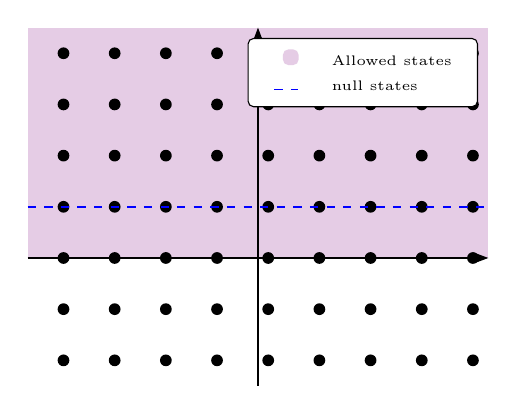
\begin{tikzpicture}[scale=0.65, font=\small]
            \def\xmin{-4.5} \def\xmax{4.5} \def\ymin{-2.5} \def\ymax{4.5}
            \clip (\xmin, \ymin) rectangle (\xmax, \ymax);
            
            \fill[violet!20] (\xmin, 0) rectangle (\xmax, \ymax);
            
            \draw[-{Stealth[]}] (\xmin, 0) -- (\xmax, 0) node[anchor=north west] {$J_0^0$};
            \draw[-{Stealth[]}] (0, \ymin) -- (0, \ymax) node[anchor=south east] {$L_0$};
            \foreach \x in {-4,...,4} {\foreach \y in {-2,...,4} {\node[dot] at (\x+0.2,\y) {};}}
            
            \draw[blue, dashed, thick] (\xmin, 1) -- (\xmax, 1);
    
            \node[draw, fill=white, rounded corners=2pt, align=left, anchor=north east, font=\tiny] at (\xmax-0.2, \ymax-0.2) {
                \begin{tabular}{rl}\tikz\fill[violet!20](0,0)rectangle(0.2,0.2);&Allowed states\\\tikz\draw[blue,dashed](0,0.1)--(0.3,0.1);&null states\\\end{tabular}};
        \end{tikzpicture}
        \caption{$\widehat{\mathcal{C}}^{\vev{1,1}}_{\alpha}$}
        \label{fig:C11_0}
    \end{subfigure}
    \hfill 
%second picture at up-right corner
    \begin{subfigure}[b]{0.48\textwidth}
        \centering
        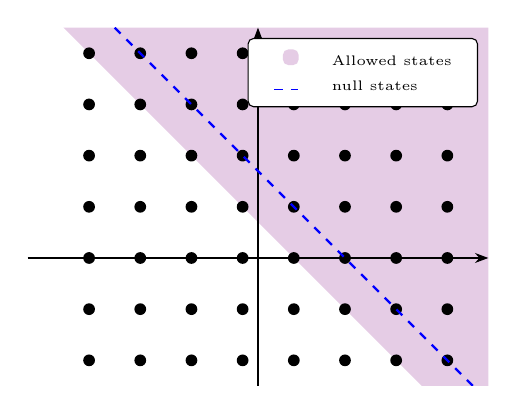
\begin{tikzpicture}[scale=0.65, font=\small]
            \def\xmin{-4.5} \def\xmax{4.5} \def\ymin{-2.5} \def\ymax{4.5}
            \clip (\xmin, \ymin) rectangle (\xmax, \ymax);

            \fill[violet!20] (-\ymax+0.7, \ymax) -- (-\ymin+0.7, \ymin) -- (\xmax, \ymin) -- (\xmax, \ymax) -- cycle;
            
            \draw[-{Stealth[]}] (\xmin, 0) -- (\xmax, 0) node[anchor=north west] {$J_0^3$};
            \draw[-{Stealth[]}] (0, \ymin) -- (0, \ymax) node[anchor=south east] {$L_0$};
            \foreach \x in {-4,...,4} {\foreach \y in {-2,...,4} {\node[dot] at (\x+0.2+0.5,\y) {};}}    
            
            \draw[blue, dashed, thick] (-\ymax+1.7, \ymax) -- (-\ymin+1.7, \ymin);
            
            \node[draw, fill=white, rounded corners=2pt, align=left, anchor=north east, font=\tiny] at (\xmax-0.2, \ymax-0.2) {
                \begin{tabular}{rl}\tikz\fill[violet!20](0,0)rectangle(0.2,0.2);&Allowed states\\\tikz\draw[blue,dashed](0,0.1)--(0.3,0.1);&null states\\\end{tabular}};
        \end{tikzpicture}
        \caption{$\widehat{\mathcal{C}}^{\vev{1,1},1}_{\alpha}$}
        \label{fig:C11_1}
    \end{subfigure}

    \vspace{1cm}

    %=====================================================
    % --- 第二行 ---
    %=====================================================

    \begin{subfigure}[b]{0.48\textwidth}
        \centering
        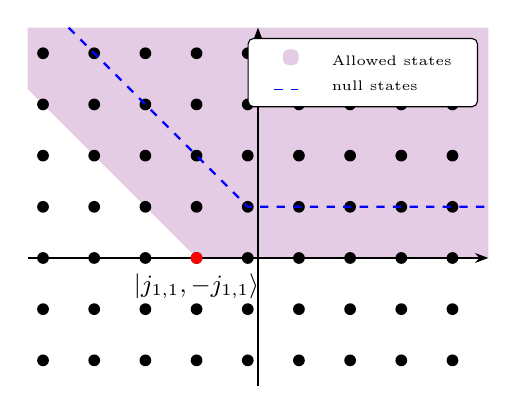
\begin{tikzpicture}[scale=0.65, font=\small]
            \def\xmin{-4.5} \def\xmax{4.5} \def\ymin{-2.5} \def\ymax{4.5}
            \clip (\xmin, \ymin) rectangle (\xmax, \ymax);

            \fill[violet!20] (\xmin, -\xmin-1.2) -- (-1.2, 0) -- (\xmax, 0) -- (\xmax, \ymax) -- (\xmin, \ymax) -- cycle;

            \draw[-{Stealth[]}] (\xmin, 0) -- (\xmax, 0) node[anchor=north west] {$J_0^3$};
            \draw[-{Stealth[]}] (0, \ymin) -- (0, \ymax) node[anchor=south east] {$L_0$};
            \foreach \x in {-4,...,4} {\foreach \y in {-2,...,4} {\node[dot] at (\x-0.2,\y) {};}}

            \draw[blue, dashed, thick] (-\ymax+0.8, \ymax) -- (-0.2, 1) -- (\xmax, 1) ;

            \node[dot, red, label=below:{$|j_{1,1}, -j_{1,1}\rangle$}] at (-1.2, 0) {};
    
            \node[draw, fill=white, rounded corners=2pt, align=left, anchor=north east, font=\tiny] at (\xmax-0.2, \ymax-0.2) {
                \begin{tabular}{rl}\tikz\fill[violet!20](0,0)rectangle(0.2,0.2);&Allowed states\\\tikz\draw[blue,dashed](0,0.1)--(0.3,0.1);&null states\\\end{tabular}};
        \end{tikzpicture}
        \caption{$\widehat{\mathcal{D}}^{\vev{1,1},\frac{1}{2}}$}
        \label{fig:D 11_1}
    \end{subfigure}
    \hfill
%fourth picture at down-right corner
    \begin{subfigure}[b]{0.48\textwidth}
        \centering
        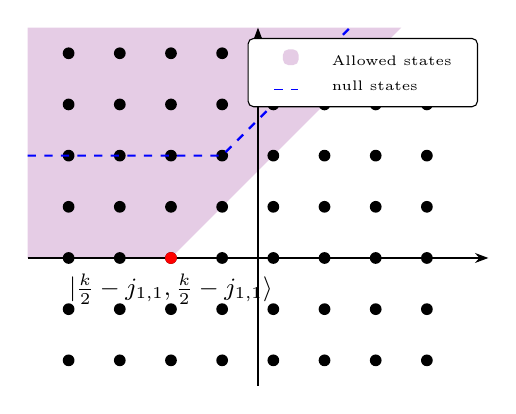
\begin{tikzpicture}[scale=0.65, font=\small]
            \def\xmin{-4.5} \def\xmax{4.5} \def\ymin{-2.5} \def\ymax{4.5}
            \clip (\xmin, \ymin) rectangle (\xmax, \ymax);

            \fill[violet!20] (\xmin, 0) -- (-1.7, 0) -- (\ymax-1.7, \ymax) -- (\xmin, \ymax) -- cycle;
            
            \draw[-{Stealth[]}] (\xmin, 0) -- (\xmax, 0) node[anchor=north west] {$J_0^3$};
            \draw[-{Stealth[]}] (0, \ymin) -- (0, \ymax) node[anchor=south east] {$L_0$};
            \foreach \x in {-4,...,4} {\foreach \y in {-2,...,4} {\node[dot] at (\x-0.7,\y) {};}}       

            \draw[blue, dashed, thick] (\xmin, 2) -- (-0.7, 2) -- (\ymax-2.7, \ymax) ;
            
            \node[dot, red, label=below:{$|\frac{k}{2}-j_{1,1}, \frac{k}{2} - j_{1,1} \rangle$}] at (-1.7, 0) {};

            \node[draw, fill=white, rounded corners=2pt, align=left, anchor=north east, font=\tiny] at (\xmax-0.2, \ymax-0.2) {
                \begin{tabular}{rl}\tikz\fill[violet!20](0,0)rectangle(0.2,0.2);&Allowed states\\\tikz\draw[blue,dashed](0,0.1)--(0.3,0.1);&null states\\\end{tabular}};
        \end{tikzpicture}
        \caption{$\widehat{\mathcal{D}}^{-1 - j_{2,1}, -}$}
        \label{fig:D 21_-1}
    \end{subfigure}

    \vspace{1cm}

        \begin{subfigure}[b]{0.48\textwidth}
        \centering
        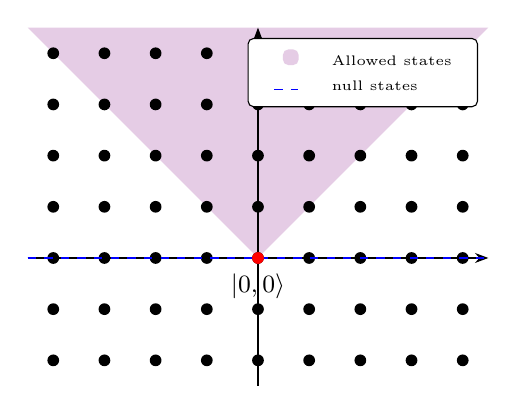
\begin{tikzpicture}[scale=0.65, font=\small]
            \def\xmin{-4.5} \def\xmax{4.5} \def\ymin{-2.5} \def\ymax{4.5}
            \clip (\xmin, \ymin) rectangle (\xmax, \ymax);

            \fill[violet!20] (\xmin, \ymax) -- (0, 0) -- (\xmax, \ymax) -- cycle;

            \draw[-{Stealth[]}] (\xmin, 0) -- (\xmax, 0) node[anchor=north west] {$J_0^3$};
            \draw[-{Stealth[]}] (0, \ymin) -- (0, \ymax) node[anchor=south east] {$L_0$};
            \foreach \x in {-4,...,4} {\foreach \y in {-2,...,4} {\node[dot] at (\x,\y) {};}}

            \draw[blue, dashed, thick] (\xmin, 0) -- (\xmax, 0) ;
            
            \node[dot, red, label=below:{$|0, 0 \rangle$}] at (0, 0) {};
                                    
            \node[draw, fill=white, rounded corners=2pt, align=left, anchor=north east, font=\tiny] at (\xmax-0.2, \ymax-0.2) {
                \begin{tabular}{rl}\tikz\fill[violet!20](0,0)rectangle(0.2,0.2);&Allowed states\\\tikz\draw[blue,dashed](0,0.1)--(0.3,0.1);&null states\\\end{tabular}};
        \end{tikzpicture}
        \caption{$\widehat{\mathcal{E}}^{1}$}
        \label{fig:E 1_0}
    \end{subfigure}
    \hfill
%fourth picture at down-right corner
    \begin{subfigure}[b]{0.48\textwidth}
        \centering
        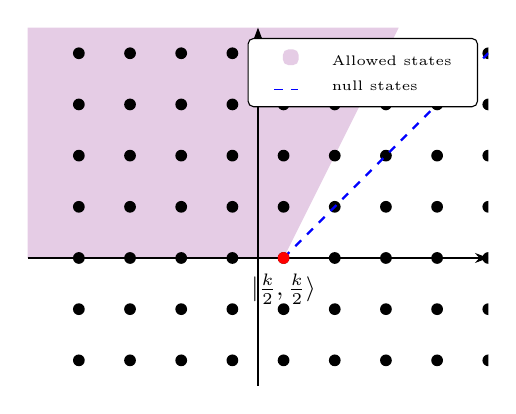
\begin{tikzpicture}[scale=0.65, font=\small]
            \def\xmin{-4.5} \def\xmax{4.5} \def\ymin{-2.5} \def\ymax{4.5}
            \clip (\xmin, \ymin) rectangle (\xmax, \ymax);

            \fill[violet!20] (\xmin, 0) -- (0.5, 0) -- (\ymax/2+0.5, \ymax) -- (\xmin, \ymax) -- cycle;
            
            \draw[-{Stealth[]}] (\xmin, 0) -- (\xmax, 0) node[anchor=north west] {$J_0^3$};
            \draw[-{Stealth[]}] (0, \ymin) -- (0, \ymax) node[anchor=south east] {$L_0$};
            \foreach \x in {-4,...,4} {\foreach \y in {-2,...,4} {\node[dot] at (\x+0.5,\y) {};}}       

            \draw[blue, dashed, thick] (0.5, 0) -- (\xmax, \xmax-0.5) ;
            
            \node[dot, red, label=below:{$|\frac{k}{2}, \frac{k}{2} \rangle$}] at (0.5, 0) {};
            
            \node[draw, fill=white, rounded corners=2pt, align=left, anchor=north east, font=\tiny] at (\xmax-0.2, \ymax-0.2) {
                \begin{tabular}{rl}\tikz\fill[violet!20](0,0)rectangle(0.2,0.2);&Allowed states\\\tikz\draw[blue,dashed](0,0.1)--(0.3,0.1);&null states\\\end{tabular}};
        \end{tikzpicture}
        \caption{$\widehat{\mathcal{D}}^{-1-j_{1,1}, -}$}
        \label{fig:E 1_-1}
    \end{subfigure}

    \caption{Spectra of degenerate representations}
    \label{fig:degrep}
\end{figure}

\section{Fusion rules}
In CFT, fusion rules form the algebra of primary fields, dictating how they combine. We could determine the fusion rules from the 
OPE 
\begin{equation}
    \phi^{j_{1},\omega_{1}}(z_{1}) \phi^{j_{2},\omega_{2}}(z_{2}) \sim 
    \vev{\phi^{j_{1},\omega_{1}}(z_{1}) \phi^{j_{2},\omega_{2}}(z_{2}) \left(\phi^{j_{3},\omega_{3}}(z_{3}) \right)^{*}} \phi^{j_{3},\omega_{3}}(z_{3}).
\end{equation}
The fusion $\widehat{\mathcal{R}}^{j_{1},\omega_{1}} \widehat{\mathcal{R}}^{j_{2},\omega_{2}} \rightarrow \widehat{\mathcal{R}}^{j_{3},\omega_{3}}$
is allowed only if the 3-point function 
$\vev{\phi^{j_{1},\omega_{1}}(z_{1}) \phi^{j_{2},\omega_{2}}(z_{2}) \left(\phi^{j_{3},\omega_{3}}(z_{3}) \right)^{*}}$ is non-zero.

On the other hand, the null vector equations give constraint on the 3-point functions involving degenerate fields. In this chapter, we 
will use the null vector equations to determine the fusion rules of degenerate representations.

\subsection{Fusion rules involving degenerate representations}

\subsubsection*{Affine primary fields}

The vanishing of null vector $\hat{N}^{c}_{1,1} \phi^{1,1}_{x} = 0$ gives the following equation:
\begin{equation}
    \vev{\hat{N}^{c}_{1,1} \phi^{1,1}_{x_{1}}(z_{1}) \phi^{j_{2}}_{x_{2}}(z_{2}) \phi^{j_{3}}_{x_{3}}(z_{3})} = 0.
\end{equation}
This equation involves operators $J^{a}_{-1}$. We substitute the local Ward identity \ref{LocalWard}, and get the following differential 
equation:
\begin{equation}
    \sum_{s=2,3} \frac{1}{z_{s1}}
    \left\{ K_{a b} D_{x_s}\left(t^a\right) D_{x_1}\left(t^c\right) D_{x_1}\left(t^b\right)+ j_{1,1} f_{a b}^c D_{x_s}\left(t^a\right) D_{x_1}\left(t^b\right) 
    - 2 j_{1,1}^2 D_{x_s}\left(t^c\right) \right\}
    \vev{\phi^{1,1}_{x_{1}}(z_{1}) \phi^{j_{2}}_{x_{2}}(z_{2}) \phi^{j_{3}}_{x_{3}}(z_{3})}  = 0. \label{nullvectoreqx}
\end{equation}
We use the conformal symmetry to send $z_{1}, z_{2}, z_{3} \rightarrow 0,1,\infty$, where only the term propotional to $\frac{1}{z_{21}}$ 
survives. Then the null vector equation corresponding to $c=-$ is simplified to 
\begin{equation}
    \begin{aligned}
        &\left\{ x_{12}^2 \partial_{1}^{2} \partial_{2} + 2 j_{2} x_{12} \partial_{1}^{2} + 2 (1-2j_{1,1})x_{12} \partial_{1}\partial_{2} \right. \\
        &\left. + 2 (1-2j_{1,1})j_{2} \partial_{1} -2j_{1,1}(1-2j_{1,1}) \partial_{2} \right\} D^{\mathbf{1}} \left[\begin{array}{ccc}
    j_{1} & j_2 & j_3 \\
    x_1 & x_2 & x_3
    \end{array} \right] = 0 .
    \end{aligned}
\end{equation}
By substituting the 3-point function in x-basis \ref{3pointfuncx}, we get the following condition on the spins: 
\begin{equation}
    \left( j_{1,1}^{2} - (j_{2}-j_{3})^{2} \right)(1+j_{1,1}+j_{2}+j_{3}) = 0.
\end{equation}
The solution to this equation is $j_{3} = j_{2} \pm j_{1,1}, -j_{2} - 1 + j_{1,1}$. Since the above equation 
is symmetric for $j_{2}$ and $j_{3}$, the other term in \ref{nullvectoreqx} proportional to $\frac{1}{z_{31}}$ should give 
the same condition. Therefore we determine the following fusion rule:
\begin{equation}
    \hat{\mathcal{R}}^{1,1} \times \hat{\mathcal{R}}^{j} = \hat{\mathcal{R}}^{j+j_{1,1}} + \hat{\mathcal{R}}^{j-j_{1,1}}.
\end{equation}
In addition, the other two null vector equations of $c = 0,+$ can be deduced from the commutation relation 
$\left[ J^{a}, \hat{N}^{b}_{1,1} \right] = \frac{ab}{c} \hat{N}^{c}_{1,1}$. Hence all three null vector equations give the 
same fusion rule. 

\subsubsection*{Spectral flowed vacuum representation}
The fusion between any representation $\hat{\mathcal{R}}^{j}$ with the vacuum representation $\widehat{\mathcal{E}}^{1}$ should give 
$\hat{\mathcal{R}}^{j}$ back: 
\begin{equation}
    \hat{\mathcal{E}}^{1} \times \hat{\mathcal{R}}^{j} = \hat{\mathcal{R}}^{j}.
\end{equation}
Hence from our assumption \ref{SpecFus}, we find 
\begin{equation}
    \rho_{\pm 1} \left( \hat{\mathcal{E}}^{1} \right) \times \hat{\mathcal{R}}^{j} = \rho_{\pm 1} \left( \hat{\mathcal{R}}^{j} \right).
\end{equation}
Let's prove this fusion rule by using the null vector appears in the spectral flowed vacuum representation, namely 
$J^{-}_{-1}\ket{-j_{1,1}-1,j_{1,1}+1}=0$. The corresponding null vector equation in $m$-basis is 
\begin{equation}
    \vev{J^{-}_{-1} \phi^{-j_{1,1}-1}_{j_{1,1}+1}(z_{1}) \phi^{j_{2}}_{m_{2}}(z_{2}) \phi^{j_{3}}_{m_{3}}(z_{3})} = 0.
\end{equation}
By using the local Ward identity, we obtain
\begin{equation}
    \begin{aligned}
        0 = &\vev{J^{-}_{-1} \phi^{j_{1}}_{m_{1}}(z_{1}) \phi^{j_{2}}_{m_{2}}(z_{2}) \phi^{j_{3}}_{m_{3}}(z_{3})} \\
        =& -\frac{1}{z_{21}} \vev{ \phi^{j_{1}}_{m_{1}}(z_{1}) J^{-}_{0} \phi^{j_{2}}_{m_{2}}(z_{2}) \phi^{j_{3}}_{m_{3}}(z_{3})} \\
        &- \frac{1}{z_{31}} \vev{ \phi^{j_{1}}_{m_{1}}(z_{1}) \phi^{j_{2}}_{m_{2}}(z_{2}) \rho_{-1}\left(J^{-}_{-1}\right) \phi^{j_{3}}_{m_{3}}(z_{3})} 
        + \frac{1}{(z_{31})^{2}} \vev{ \phi^{j_{1}}_{m_{1}}(z_{1}) \phi^{j_{2}}_{m_{2}}(z_{2}) \rho_{-1}\left(J^{-}_{0}\right) \phi^{j_{3}}_{m_{3}}(z_{3})}.
    \end{aligned}
\end{equation}
Substituting the global Ward identity \ref{GlobalWard}to the above null vector equation, 
we find the null vector equation is simplified to 
\begin{equation}
    (\frac{1}{z_{21}}- \frac{1}{z_{31}}) \vev{ \phi^{j_{1}}_{m_{1}}(z_{1}) J^{-}_{0} \phi^{j_{2}}_{m_{2}}(z_{2}) \phi^{j_{3}}_{m_{3}}(z_{3})} - 
    \frac{1}{(z_{31})^{2}} \vev{ \phi^{j_{1}}_{m_{1}}(z_{1}) \phi^{j_{2}}_{m_{2}}(z_{2}) \rho_{-1}\left(J^{-}_{0}\right) \phi^{j_{3}}_{m_{3}}(z_{3})} = 0.
\end{equation}
Substitute the spectral flow violating 3-point function \ref{3pointfunc_m-1}. 
Since $\Delta^{j_{3},-1}_{m3-1} = \Delta^{j_{3},-1}_{m_{3}} - 1$, we find the $z$-dependence of these two terms is exactly the same. 
The equation is simplified to 
\begin{equation}
    (-j_{2}-1+m_{2}) (m_{2}+j_{2}) - (-j_{3}-1+m_{3}) (m_{3}+j_{3}) = 0.
\end{equation}
Since the $m$ is conserved, we have $m_{3} = -m_{2} + 1$. We find the above equation has only two solutions $j_{3} = j_{2}, -j_{2}-1$. 
Hence we proved that 
\begin{equation}
    \rho_{1} \left(\widehat{\mathcal{E}}^{1}\right) \times \widehat{\mathcal{R}}^{j} = \rho_{1} \left( \hat{\mathcal{R}}^{j} \right).
\end{equation}

\subsubsection*{Generic spectral flowed representations}
The above fusion rule involving vacuum representations can be generalized to generic level 1 degenerate representations. 
The null vector at level 1 gives the following equation:
\begin{equation}
    \vev{J^{+}_{-1} \phi^{\vev{1,1}}_{m_{1}-1} \phi^{j_{2}}_{m_{2}}(z_{2}) \phi^{j_{3},-1}_{m_{3}}(z_{3})} 
    + 2\vev{J^{0}_{-1} \phi^{\vev{1,1}}_{m_{1}} \phi^{j_{2}}_{m_{2}}(z_{2}) \phi^{j_{3},-1}_{m_{3}}(z_{3})} 
    - \vev{J^{-}_{-1} \phi^{\vev{1,1}}_{m_{1}+1} \phi^{j_{2}}_{m_{2}}(z_{2}) \phi^{j_{3},-1}_{m_{3}}(z_{3})} = 0.
\end{equation}
Substituting the local Ward identity, the equation is equivalent to 
\begin{equation}
    \begin{aligned}
        0 = & \frac{1}{z_{21}}\vev{ \phi^{\vev{1,1}}_{m_{1}-1} J^{+}_{0} \phi^{j_{2}}_{m_{2}}(z_{2}) \phi^{j_{3},-1}_{m_{3}}(z_{3})}  
        +2\frac{1}{z_{21}}\vev{\phi^{\vev{1,1}}_{m_{1}} J^{0}_{0}\phi^{j_{2}}_{m_{2}}(z_{2}) \phi^{j_{3},-1}_{m_{3}}(z_{3})} \\
        & +2\frac{1}{z_{31}}\vev{\phi^{\vev{1,1}}_{m_{1}} \phi^{j_{2}}_{m_{2}}(z_{2}) J^{0}_{0}\phi^{j_{3},-1}_{m_{3}}(z_{3})} 
        -\frac{1}{z_{21}}\vev{\phi^{\vev{1,1}}_{m_{1}+1} J^{-}_{0}\phi^{j_{2}}_{m_{2}}(z_{2}) \phi^{j_{3},-1}_{m_{3}}(z_{3})}\\ 
        & - \frac{1}{z_{31}}\vev{\phi^{\vev{1,1}}_{m_{1}+1} \phi^{j_{2}}_{m_{2}}(z_{2}) \rho_{-1}\left(J^{-}_{-1}\right)\phi^{j_{3},-1}_{m_{3}}(z_{3})} 
        +\frac{1}{(z_{31})^{2}}\vev{\phi^{\vev{1,1}}_{m_{1}+1} J^{-}_{0}\phi^{j_{2}}_{m_{2}}(z_{2}) \rho_{-1}\left(J^{-}_{0}\right)\phi^{j_{3},-1}_{m_{3}}(z_{3})} .
    \end{aligned}
\end{equation}
Substituting the 3-point function, again we find the $z$-dependence cancels and the equation reduces to 
\begin{equation}
    (-j_{1,1}-1+m_{1}+2m_{2})(-j_{1,1}+m_{1}) - (m_{3}-m_{2})((1-m_{3}-m_{2})) = 0.
\end{equation}
Since we have $j_{1,1} = -\frac{k+2}{2}$ and $m_{1}+m_{2}+m_{3}+\frac{k}{2}$, we find the above equation is simplified to :
\begin{equation}
    j_{2}(j_{2}+1) - j_{3}(j_{3}+1) = 0.
\end{equation}
We find two solutions: $j_{2} = j_{3},-j_{3}-1$, which gives the following fusion rule:
\begin{equation}
    \widehat{\mathcal{R}}^{\vev{1,1}} \times \widehat{\mathcal{R}}^{j} \supset \rho_{1} \left( \widehat{\mathcal{R}}^{j} \right).
\end{equation}
The fusion rule should be symmetric for $\rho_{\pm 1}$, hence we should also have 
\begin{equation}
    \widehat{\mathcal{R}}^{\vev{1,1}} \times \widehat{\mathcal{R}}^{j} \supset \rho_{-1} \left( \widehat{\mathcal{R}}^{j} \right).
\end{equation}

In conclusion, we conjecture the fusion rule between a degenerate representation and a generic affine highest weight representation to be: 
\begin{equation}
    \widehat{\mathcal{R}}^{\vev{1,1}} \times \widehat{\mathcal{R}}^{j} = \widehat{\mathcal{R}}^{j+j_{1,1}} \oplus \widehat{\mathcal{R}}^{j-j_{1,1}}
    \oplus \rho_{1} \left( \widehat{\mathcal{R}}^{j} \right) \oplus \rho_{-1} \left( \widehat{\mathcal{R}}^{j} \right).
\end{equation}


\printbibliography
\end{document}